\documentclass[12pt, english, NoHyper]{AE4010-template}
\usepackage[]{natbib}
% \usepackage[sorting=none, citestyle=numeric-comp, natbib=true]{biblatex}    % For numbered biblatex references
%  \usepackage[citestyle=authoryear]{biblatex}      % For author year biblatex references
\usepackage{csquotes}
\usepackage{hyperref}
\usepackage{amsmath}
\usepackage{graphicx}
\usepackage{lscape}

\renewcommand{\baselinestretch}{1.0}
\setlength{\parskip}{-0.2em}


%% Uncomment the following three lines when using the biblatex package
%\bibliography{bibliography.bib}
%\addbibresource{bibliography.bib}
%\bibliography{apa}
%% Uncomment the following line when using the natbib package
\bibliographystyle{plainnat}





%% Define your title entries here
\title{Identification of Potentially Hazardous Asteroids}
\author{J. G. P. Vermeulen}
\yourstudynumber{4382889}
\yourmscprofile{Space Flight}
\yourmsctrack{Space Systems Engineering}









%   ########################################################################
%               PLEASE COMPILE USING XELATEX FOR THE BEST RESULTS
%   ########################################################################









\begin{document}
\maketitle

\section*{Executive Summary}
A research project is proposed to investigate capabilities and properties of a space-based Near-Earth Asteroid (NEA) survey using a system of multiple satellites. In recent years, several research projects have investigated deep space NEA surveys using single spacecraft, in order to improve the fraction of known NEAs smaller than 140 meter, as well as the warning time before impact. The research proposed here aims to investigate the influence of the number of spacecraft in a space-based survey through detailed simulation of Near-Earth Asteroid surveys. By modelling asteroid surveys, the relations and behavior of such missions will be mapped out. In addition, optimization will be performed to compare the capabilities of such missions to current NEA surveys. As the first research into multi-satellite NEA surveys, this work will provide the groundwork for more detailed research into specific missions which can further humanity's protection against asteroid impacts, as well as its understanding of the smaller bodies in the Solar system.




\section{Introduction}
In recent years, human efforts have catalogued all very large near-Earth asteroids and determined none of these to be a threat in the foreseeable future. However, as illustrated by recent impacts such as the Chelyabinsk and Tunguska meteors, smaller, unknown, asteroids still pose a significant threat to human life and property. In addition, an upscaling of Earth-based detection methods will not suffice to safeguard humanity from these natural disasters: unfavorable phase angles and atmospheric interference make detection from the Earth inefficient (\cite{DefendingPlanetEarth}). In recent years, a multitude of studies (e.g. \cite{NEOSDT1}, \cite{ThesisOlga}) have been performed to assess the effectivity of a future space-based Near-Earth Object surveying mission. These studies have yielded promising results, but still suffer from some additional issues, such as interference by sunlight and limitation on data processing. Therefore, a system of detection is proposed based on autonomous satellites placed strategically in the solar system to automatically detect near-Earth asteroids and identify whether these are impact-hazardous to Earth. Next to increasing the amount of data gathered, a multi-spacecraft system has two distinct advantages: it allows for a diversity of viewing angles, decreasing interference by the Sun; and it allows for more, distributed computational power for processing data in space. Despite these advantages, so far no research has been carried out concerning such a system.\\

This work contains a project plan for proposed research into the topic of multi-satellite asteroid surveys. Firstly, an overview of the current state of literature, and the position of the work therein is discussed. Next, the core of the research as intended is described, starting with the research question, aim and subgoals; followed by the methodology, setup of the experimentation, and expected outcomes. Lastly, a short discussion of the project plan will be given.







\section{State-of-the-art/Literature Review}
Study of Potentially Hazardous Asteroids (PHA's) began through initiatives from governments to safeguard Earth from the threat of asteroid impacts, resulting in several of the foundations of the field (\cite{InitialTaskforce}, \cite{DefendingPlanetEarth}). These agreed upon the initiative to identify 90\% of all Near-Earth Asteroids\footnote{Defined as an asteroid with perihelion < 1.3 AU} larger than 140 m in diameter. This was based on the calculation that this would eliminate 90\% of the remaining background impact risk. Thus, the PHA was defined as an asteroid with a diameter over 140 meter, which intersects Earth's orbit within 0.05 AU. \\

In the following years, a multitude of surveys were carried out to achieve this goal, such as, but not limited to, the Catalina Sky Survey and the PANSTARRs survey in Hawaii. In addition, several surveys were carried out from space, most notable the NEOWISE survey which repurposed the WISE imager after its main cryogenic payload had run out. The performance of these surveys has been spectacular (see e.g. \cite{NEOWISEFlex}). However, as shown by \cite{PopulationHarris} in \autoref{fig:populationdifference}, a large fraction of asteroids is still unknown.\\

\begin{figure}[thb]
 \centering
 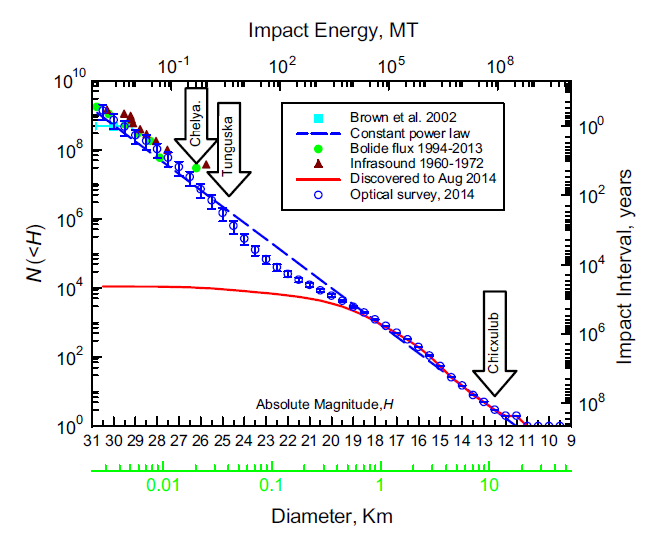
\includegraphics[width=0.8\textwidth]{figures/populationdifference.png}
 \caption{Relationship between asteroid absolute magnitude (and thus size, and impact energy) to their occurence. Shown are the expected comulative population of these asteroids (listed as the number \textit{N} with absolute magnitude < \textit{H}), compared to the number discovered in contemporary surveys. \cite{PopulationHarris}}
 \label{fig:populationdifference}
\end{figure}

As the remaining fraction of asteroids not only poses a threat to human safety and property, but discovering them will also yield valuable scientific insights into the structure and origin of our solar system (\cite{Populations}), a number of new surveys is currently being researched and developed. Among the ground-based surveys, the most ambitious current project is the Large Synoptic Survey Telescope at the Vera C. Rubin observatory in Chile (see \cite{LSST} for a thorough overview). However, as Earth-based surveys are limited by weather, day/night cycles and atmospheric dispersion, most of the research is focussed on space-based surveys. \\

Although the efficacy of Earth-orbiting missions has already been shown by missions such as the Spitzer space telescope and NEOWISE, there is currently a lot of interest in deep space surveys. Advantages of these surveys include not being influenced by sunlight reflected off Earth, more favourable viewing angles, and greater relative motion to the asteroids (\cite{NEOSDT1}). The largest barrier to performing these missions, the lack of sufficient computational power, has been resolved by advances in semiconductor technology. However, because of the vast costs of a space mission, most work is currently focussed on simulating surveys to determine optimal conditions, such as the work done at the European Space Agency by \cite{Flyeye} and at NASA Jet Propulsion Laboratory by \cite{NEOSDT2}. \\

Investigation of the possibilities yields that space-based surveys will be superior the current Earth-based surveys. Commonly researched orbits are Earth-Sun L1, Venus-Sun L1, Venus-trailing, and several Earth orbits, using either visual light or thermal infrared telescopes (see e.g. \cite{NEOSDT1}). \cite{ThesisOlga} expands on these even further by showing advantages of using solar sails for more complex orbits. Although the performance of these surveys is impressive, there is still a large number of PHAs that will not be found by these surveys, and an even larger fraction of smaller NEAs that will remain undiscovered, as shown by \cite{NEOSDT2} in \autoref{fig:surveycompleteness}. Therefore, in this report, a proposal will be made to research if the performance of these surveys can be improved through utilization of a system of several satellites, hoping to exploit a greater variety in orbits, payload combinations, and viewing angles.

\begin{figure}[thb]
 \centering
 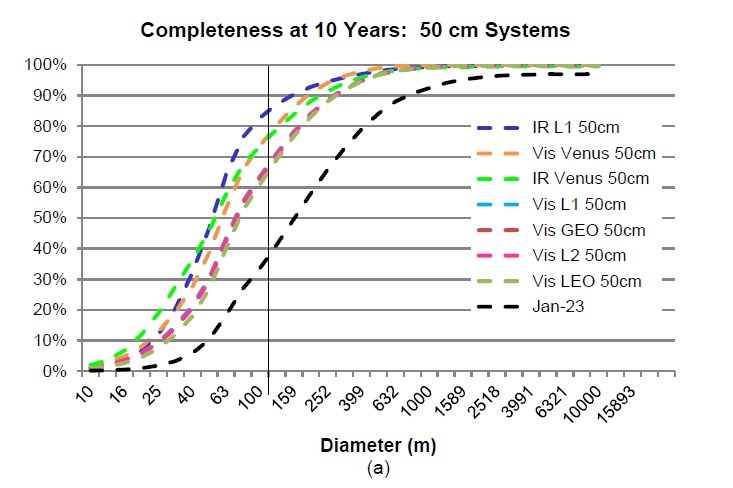
\includegraphics[width=0.8\textwidth]{figures/surveycompleteness.png}
 \caption{Survey completeness at 10 years, using 50cm telescopes. Simulation by \cite{NEOSDT2}.}
 \label{fig:surveycompleteness}
\end{figure}


\section{Research Question, Aim/Objectives and Sub-goals}
As there is currently no established baseline for multi-satellite asteroid surveys, the research will focus on examining how such a survey would compare to existing, more well studied proposals.

\subsection{Research Question}
Therefore, the research question of this work is:

\begin{quote}
 How is the performance, optimal position and configuration of a space-based system with the purpose of identifying and cataloguing near-Earth objects affected by the number of spacecraft in the system?
\end{quote}

As briefly alluded to previously, there are actually two objectives of such a survey: raising the ``survey completeness'', i.e. what fraction of asteroids is known, and raising the warning time for impactors heading towards Earth by identifying them early. Therefore, the following two sub-questions are identified:

\begin{quote}
 How does the number of said spacecraft affect a system with the purpose of raising the warning time for Earth impactors?
\end{quote}
\begin{quote}
 How does the number of said spacecraft affect a system with the purpose of raising the survey completeness of near-Earth asteroids?
\end{quote}

And lastly, a tangential question that will be a crucial component of the main project:

\begin{quote}
 What is the influence of a system utlizing mixed infrared and visual telescopes to perform said survey?
\end{quote}

This final question is often suggested as future work by authors (e.g. \cite{AsteroidsInTIR}, \cite{AsteroidSTM}), and should be investigated independently to ensure a proper interpretation of the configuration of the system.

\subsection{Research Objective}
As mentioned previously, modern research into this topic is carried out through detailed modelling of surveys using computers. Therefore, the main research objective of this thesis is:

\begin{quote}
To investigate the influence of the number of satellites in a space-based survey through detailed simulation of near-Earth asteroid surveys.
\end{quote}

The first of the sub-objectives is to accurately model the asteroid population. Several alternatives exist for this, but it is important to consider the implications of how the models were constructed, given that none of them was based on a deep space survey.\\

The second sub-objective is to accurately model the survey of this population. For this, three issues have to be addressed: Firstly, the signal generated by the asteroid has to be modelled. Secondly, the background signal and noise has to be modelled. With these two objectives completed, a suitable survey cadence should then be derived to integrate the survey in time.\\

Lastly, the ``optimal'' part of the survey. As the satellites are not bound to a single position, options such as L1 points are no longer a de-facto preferred location. Therefore, a method is necessary to determine what the optimal placement and composition of such a system is. Most likely, this will be the most computationally intensive part, as the complexity of the problem quickly grows when increasing the size of the system.

\section{Theoretical Content/Methodology}
In this section, the methodology for the three sub-objectives stated above is laid out.

\subsection{Asteroid Population}
%https://www.mv.helsinki.fi/home/mgranvik/data/Granvik+\_2018\_Icarus/
%https://www.sciencedirect.com/science/article/pii/S0019103517307017?via\%3Dihub#fn0003
Several peer-reviewed and validated models of the NEA population exist, which can be used easily for the intended research. It is important to assess the model using different population models, to ensure generalization of the solution. For a full population model, intended to assess the identification and cataloguing performance, two models have been selected. The first model is the de-biased model by \cite{PopulationGranvik}. This model continues on the work of \cite{PopulationHarris}, as well as the results of the NEOWISE mission. It derives an algorithmic model which can directly generate a representative population of NEAs. In addition to this model, the real database of NEAs gathered by NASA/JPL will be used (\cite{CNEOSDatabase}). Although this model is biased, as it only includes asteroids that were discovered already, it is known to be a correct representation of reality, as it is not simulated.\\

As asteroid impacts are rare, assessing the warning time requires a population of synthetic impactors. Using various methods, several authors have created and succesfully used populations of synthetic impacts, with representative orbital elements to actual impactors. The standard among these models is the model by \cite{ChelseyPop}. This model includes orbital elements for a large population of asteroids, as well as predicted time of impact. In addition, the model developed by \cite{Flyeye} will be used, which has been applied in this fashion in the past successfully by \cite{ThesisOlga}.\\

Lastly, in order to determine the position of the asteroids in time from their orbital elements, simple Keplerian orbits will be used, as precise accuracy of the orbits is not neccessary for the inteded research. This will save a lot of computational power in optimization.


\subsection{Survey Modelling}
Modelling of the survey is by far the largest part of the initial set-up work. The survey can be split up into three categories: Modelling the background signal and noise, modelling the signal from the asteroids, and modelling the cadence and detection by the satellite. As mentioned previously, both visual light and thermal infrared will be considered. Therefore, models need to be developed for both.

\subsubsection{Background Signal and Noise}
There are a lot of components to the background signal: Diffuse starlight from the night sky, a concentration of background light along the plane of the Milky Way, the direct light of the Sun, the zodiacal light, and the so-called gegenschein (specular reflection of light off of dust directly opposite the Sun). For simplicity, these components are split into a Solar and a galactic component. The Solar component is dependent on the location of the satellite around the Sun; the galactic component is not. \\

For the visual light, implementation is simple. Detailed measurements have been taken of the visual background light, see e.g. \cite{LightOfTheNightSky}. These values have been tabulated by \cite{DiffuseSkyBrightness}, split into Solar and galactic components. These have been verified and can be directly implemented. \\

The thermal infrared signal is slightly more complicated, as the contribution of zodiacal light is not mainly dependent on reflection, but on the temperature distribution of interplanetary dust, which varies throughout the Solar system. The most complete model available currently is based on the COBE mission, as described by \cite{COBEIRBackground}. This model is split up into detailed measurements of the galactic IR background, combined with a model of interplanetary dust. This model can be integrated numerically to find the contribution of interplanetary dust and solar radiation. \\

Lastly, there are several noise terms inherent to the detector. These are mainly read noise and thermal noise. The values for these are hardware dependent and were taken from \cite{NEOSDT2}. In addition, because of the nature of a signal consisting of individual particles, there is a contribution of Poisson noise in all terms.

\subsubsection{Target Signal}
Determination of the target signal in the visual light is straightfoward: by assuming the asteroid is approximately a diffusely reflecting sphere, the standard phase function given by Lambert's cosine law can be used. However, no such phase function has been found in the infrared spectrum. The basis for the infrared signature of an asteroid was given by \cite{AsteroidSTM}: By making an assumption on the temperature distribution of the asteroid, based on its thermal balance, a numerical integration of the visible hemisphere is performed for the flux. This model was later refined by \cite{AsteroidsInTIR} using data from a larger number of asteroids. Their Near-Earth Asteroid Thermal Model (NEATM) will be used in the experiment.

\subsubsection{Cadence and Detection}
Detection of NEAs is contingent on several repeat measurements. These \textit{tracklets} can then be combined to fit the orbital elements (\cite{OpNav}). Therefore, how often a measurement is taken is of relevance. In order to determine the frequency of measurements, the \textit{cadence}, an analysis of the ADCS will be performed together with the required integration time of the camera (from \cite{NEOSDT2} and \cite{ThesisOlga}). \\

To establish a detection, a signal-to-noise ratio calculation will be performed. This saves a lot of computational load compared to processing generated images. The SNR can be calculated according to \cite{NEODetection} as follows:
\begin{equation}
\mathrm{SNR} = \frac{\frac{1}{hc}A\tau k_{sf} \int_{\lambda_1}^{\lambda_2}E_A(\lambda)Q_e(\lambda)T(\lambda)\lambda d \lambda}{\sqrt{S_e + B_e + D_e + R_e^2}}
\end{equation}
With target and background signal in electrons $S_e$ and $B_e$, dark noise $D_e$ and read noise $R_e$. The remaining terms are largely efficiency terms, the interested reader is refered to \cite{NEODetection} or \cite{OpNav} for a thorough explanation. Note that only the poisson component of the background signal has to be taken into account, as the mean signal can be subtracted easily (\cite{OpNav}).\\

To convert a SNR to a detection, a probabilistic approach is taken. A lower threshold of SNR = 1 is set (0\% chance of detection), and a higher threshold of SNR = 5 (100\% detection). Between these thresholds, an integrated Gaussian is used to determine the detection probabilistically. 3 detections within a time span of 90 days will lead to the asteroid being identified (\cite{NEOSDT1}). Lastly, by numerically working through this model in time, the performance of the full asteroid survey can be modelled.

\subsection{Optimization}
To judge the capabilities of the system as a function of the number of satellites, the optimal position and composition has to be determined. As little is known about the behavior of the system, there is no simple mathematical model available to perform this optimization. Therefore, a numerical approach is required. \\

Initially, some exploration of the behavior of the system will be performed. At this stage, too little is known about the system to select a proper optimization algorithm. Therefore, the first stage of research will use a coarse grid search, as detailed in \cite{DLOne}. In a grid search, all variables are iterated over at a preset interval. All performance metrics will be recorded, and the highest score will present the optimal solution. \\

When initial data is available to assess the behavior of the system, it is possible to select a proper optimizer for further research. Due to the nature of the model, it is expected that some form of heuristic optimization will be required. This class of methods uses a heuristic to approximate the optimal solution, rather than converging mathematically. As a result, they can be significantly faster when applied properly, and they can be applied to more diverse problems. Common methods that will be traded off include, but are not limited to, genetic algorithms, simulated annealing and particle swarm optimization. These methods are extensively documented by e.g. \cite{DLTwo} and \cite{DLOne}.


\section{Experimental Set-up}
As explained in the methodology section, experiments will be ran purely numerically on computers. All simulations will be created in Python 3, for the following reasons: Firstly, Python offers a wide framework of advanced optimization tools, and data analysis toolkits. In addition, Python is simple to work with and validate, as it is an interpreted language. It thus allows for easy iteration. Lastly, the author is highly familiar with Python 3 and the relevant packages. \\

The main packages that will be used are the data handling package \textit{Pandas}, which allows for object-oriented style handling of large amounts of data in-memory. For optimization, the preferred packages are Scikit-Learn and Tensorflow, both of which allow for out-of-the-box application of algorithms as they are described by e.g. \cite{DLOne}. Importantly, both these packages are widely used, and their implementation has been thoroughly reviewed. The former allows for executing the code on CPU cores. The latter also supports GPU acceleration through CUDA, if neccessary. Data visualisation will be performed using Seaborn, a wrapper for Matplotlib. \\

To run the simulation, the author has access to several modern desktop computers equiped with 6-core AMD Ryzen 3600 processors, and Nvidia graphics cards supporting CUDA (ranging from 1408-core GTX1660 Super to 1920-core RTX2060). Initially, it is expected that this will suffice to generate results in a relatively quick manner. In addition, a request will be made to the department of Astrodynamics and Space Missions for access to their compute cluster. This cluster will be used in later stages of research where more computationally intensive simulations will be ran.


\section{Results, Outcome and Relevance}
Starting from the research question, the topics of interest are the performance, optimal position, and configuration of the space system. The main dependent variable is the performance, which will be assessed in two ways: The first and primary objective is the \textit{survey completeness}, the fraction of asteroids which is detected after a survey. The secondary objective is the \textit{warning time} of impacting asteroids, measured in the number of days before impact that the asteroid is found. This will be assessed relative to the current performance of warning systems such as ATLAS. \\

Primarily, the research aims to show what the effects are of changing the position and configuration - both in payload and in number - of the sytem on its performance. Through this, in the future more advanced missions may be considered which will advance the knowledge of the NEA population as much as possible. Specific results which are of particular interest are listed in the following paragraphs. \\

Firstly, the effect on performance when increasing the number of satellites. It is expected that the performance will increase with every added satellite. In addition, two effects are hypothesized: firstly, due to the nature of orbit determination (instead of solving Gauss' problem with observations from a single satellite, using multiple satellites allows for triangulating the position, and solving Lambert's problem instead), it is expected that a synergistic effect will appear for low numbers of satellites. Secondly, as it is highly unlikely that performance will scale linearly with the number of satellites, it follows logically that there will be a form of diminishing returns for higher numbers of satellites. \\

In addition to the primary performance of the system, the other parameters of interest are the optimal values of the independent variables in the optimization. This will give insights into how, for example, the optimal semi-major axis of the mission's orbit evolves when the number of satellites in the system increases. It is expected that, as more satellites allow for more spreading out, the optimal semi-major axis will increase as the number of satellites increases. Additionally, this will allows evaluation of the performance and interaction of the various payloads. \\

Because of the complex nature of the simulation, verification and validation are essential to ensure robust results. This is further complicated by the application of heuristic-based optimization methods, which can be prone to overfitting the data (\cite{DLOne}). Verification of the software will be performed through standard verification practices: during programming unit tests of the various functions and subfunctions will be performed, supplemented by code review. Validation will be performed through comparison of the (partial) outputs of the simulations to results presented in literature. Most of the components of the models originate in articles, which often include examples of their results. Replication of these results should be checked. For the full system, the results will be compared by simulating surveys similar to those performed by \cite{NEOSDT2}. The performance of these surveys should be a replication of the results from literature, without prejudice to small deviations originating from changes in implementation. Lastly, there are several steps to ensure a robust generalization of the optimization. Mainly, several datasets or selections from datasets should be evaluated per solution. This ensures that the optimization will not overfit to the population or survey models, but will provide insights into the underlying problem as intended. The results should also be closely inspected for this, and compared to a validation set which was not used prior to or during optimization (see e.g. \cite{DLTwo} for best practices regarding robustness of these models).

In the end, the research will provide relations between the various parameters in such a complex system. Although no exact design of a mission can be given, these relations can be used as a starting point for designing the asteroid survey missions of the future.


\section{Project Planning and Gantt Chart}
In any project, proper planning is extremely important in order to avoid delays and ensure a smooth execution of the plans. To this end, a work breakdown will be performed, from which a Gantt chart will be constructed.
\subsection{Work Breakdown}
The work is broken down into nine phases. These phases are ordered in order of execution, although there is some overlap between the various phases. This will be further shown in the Gantt chart. The phases are as follows:
\begin{enumerate}
\setlength\itemsep{-0.5em}
 \item \textbf{Mission}: Firstly, it needs to be made clear exactly \textit{what} the problem is that needs to be adressed, and \textit{how} it will be tackled.
 \item \textbf{System description and boundaries}: Then, the system will be analysed to find the relevant boundaries, define the scope of the research, and identify and key requirements and constraints.
 \item \textbf{Asteroid population modelling}: After the initial examination of the mission and system, the modelling will begin. The first part of the model, the asteroid population, will be largely performed from sources in literature, as explained in the methodology section.
 \item \textbf{Survey modelling}: The largest part of the modelling effort concerns the survey modelling, with both target signal calculations as well as background and noise calculations, combined with survey-specific properties following from the mission and system description.
 \item \textbf{Optimization}: Based on examination of the initial properties of the system, an optimization method will be selected and implemented to find the best possible solutions to the problem.
 \item \textbf{Research}: Parameters and quantities of interest have to be examined to explore the properties of the system. This ranges from deriving simple 1-to-1 relations between variables, to complex multi-dimensional simulations. Covering the relevant parts of the solution space is essential for making sure all aspects of the problem are explored.
 \item \textbf{Analysis}: The research phase will generate a large quantity of data. This data has to be analysed, both qualitatively as well and quantitatively. Through this, a robust understanding of the problem can be formulated, and conclusions can be drawn which are useful in designing future missions.
 \item \textbf{Reporting}: All phases need to be adequately documented, supported and explained. The process of reporting should be simultaneous with the work, and should not be left for the last moment.
 \item \textbf{Presentation}: Finally, a public defense of the work performed needs to be prepared and delivered.
\end{enumerate}

To convert this work to a Gantt chart, it is considered what activities depend on each other. This is vital to ensure no delays occur when a part of the work gets stuck, or is performed too late. There are a few main drivers to ensuring this happens swiftly: At first, the simulation has to be developed. No research work can be carried out before this is done, and as such it is vital to finish this as soon as possible. As running the simulations can take a considerable amount of time, the simulations should be validated before it is used, not afterwards. Then, when running the simulations, the results can be examined in parallel. Examining these results allows for an iterative process: interesting relations are found, and from there more targeted research can be performed. In addition, some exploration will need to take place before a suitable optimizer can be selected. Lastly, all work needs to be done in time for the relevant milestones (Kick-off, Mid-term review and Green-light review), as well as in time to allow for reporting. The work breakdown structure can be found in \autoref{sec:WBS} and the Gantt chart in \autoref{sec:Gantt} The dates for the relevant milestones are set as follows:
\begin{itemize}
\setlength\itemsep{-0.5em}
 \item Kick-off meeting: 9 August 2021
 \item Mid-term review: 12 November 2021
 \item Green-light review: 28 January 2022
 \item Hand-in thesis: 14 February 2022
 \item Defense and graduation: 28 February 2022
\end{itemize}


\section{Conclusions}
Through this research proposal, insight will be gained into the properties of multi-satellite space systems aimed at improving the survey completeness of NEAs and increasing the warning time of Earth-impacting NEAs. A detailed simulation comprised of a visual and thermal infrared background signal, target signal, and representative noise parameters will be created. Using this simulation, the influence of the main parameters of a multi-satellite asteroid survey mission will be investigated. In addition, optimization will be performed to obtain an indication of the best possible performance. Ultimately, this will provide a trade-off of such a multi-satellite system to the current and past space-based mission proposals and capabilities, ultimately broadening the possibilities for planetary defence and solar system science.

\newpage
%% Use letters for the chapter numbers of the appendices. 
%% Note: when there are references in the appendices, the references should be placed below the appendices.
\appendix
%% Uncomment the following line when using the natbib package
\bibliography{bibliography.bib}

%% Uncomment the following line when using the biblatex package
% \printbibliography
\newpage
\begin{landscape}
 \section{Work Breakdown Structure}
 \label{sec:WBS}


\begin{figure}[h!]
 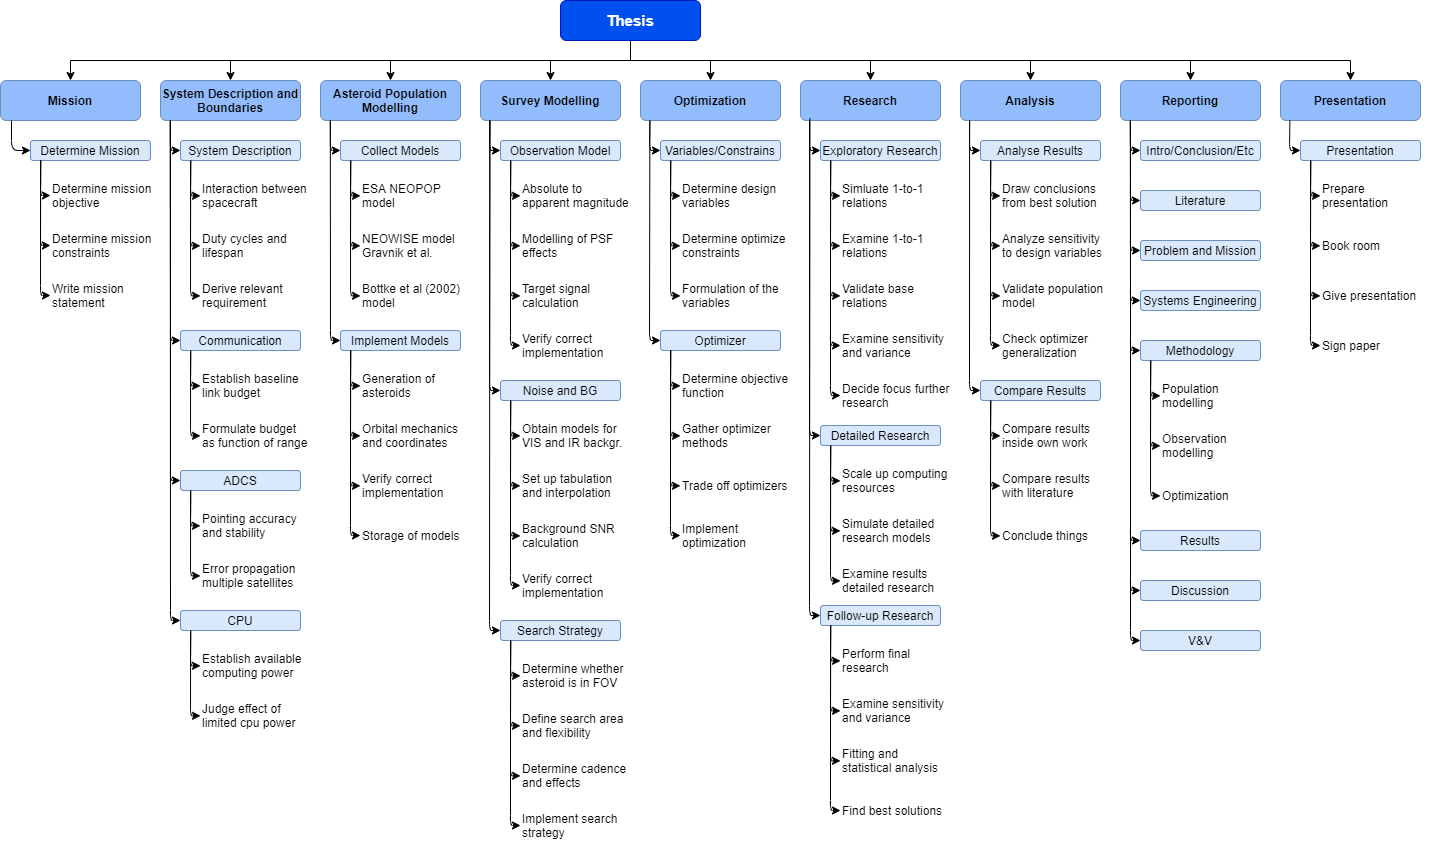
\includegraphics[width=1.0\textwidth]{figures/wbs.png}
\end{figure}
Full resolution link: \url{https://surfdrive.surf.nl/files/index.php/s/WY60MXT6ajXHEfp}
\end{landscape}
\newpage
\begin{landscape}
 \section{Gantt Chart}
 \label{sec:Gantt}


\begin{figure}[h!]
 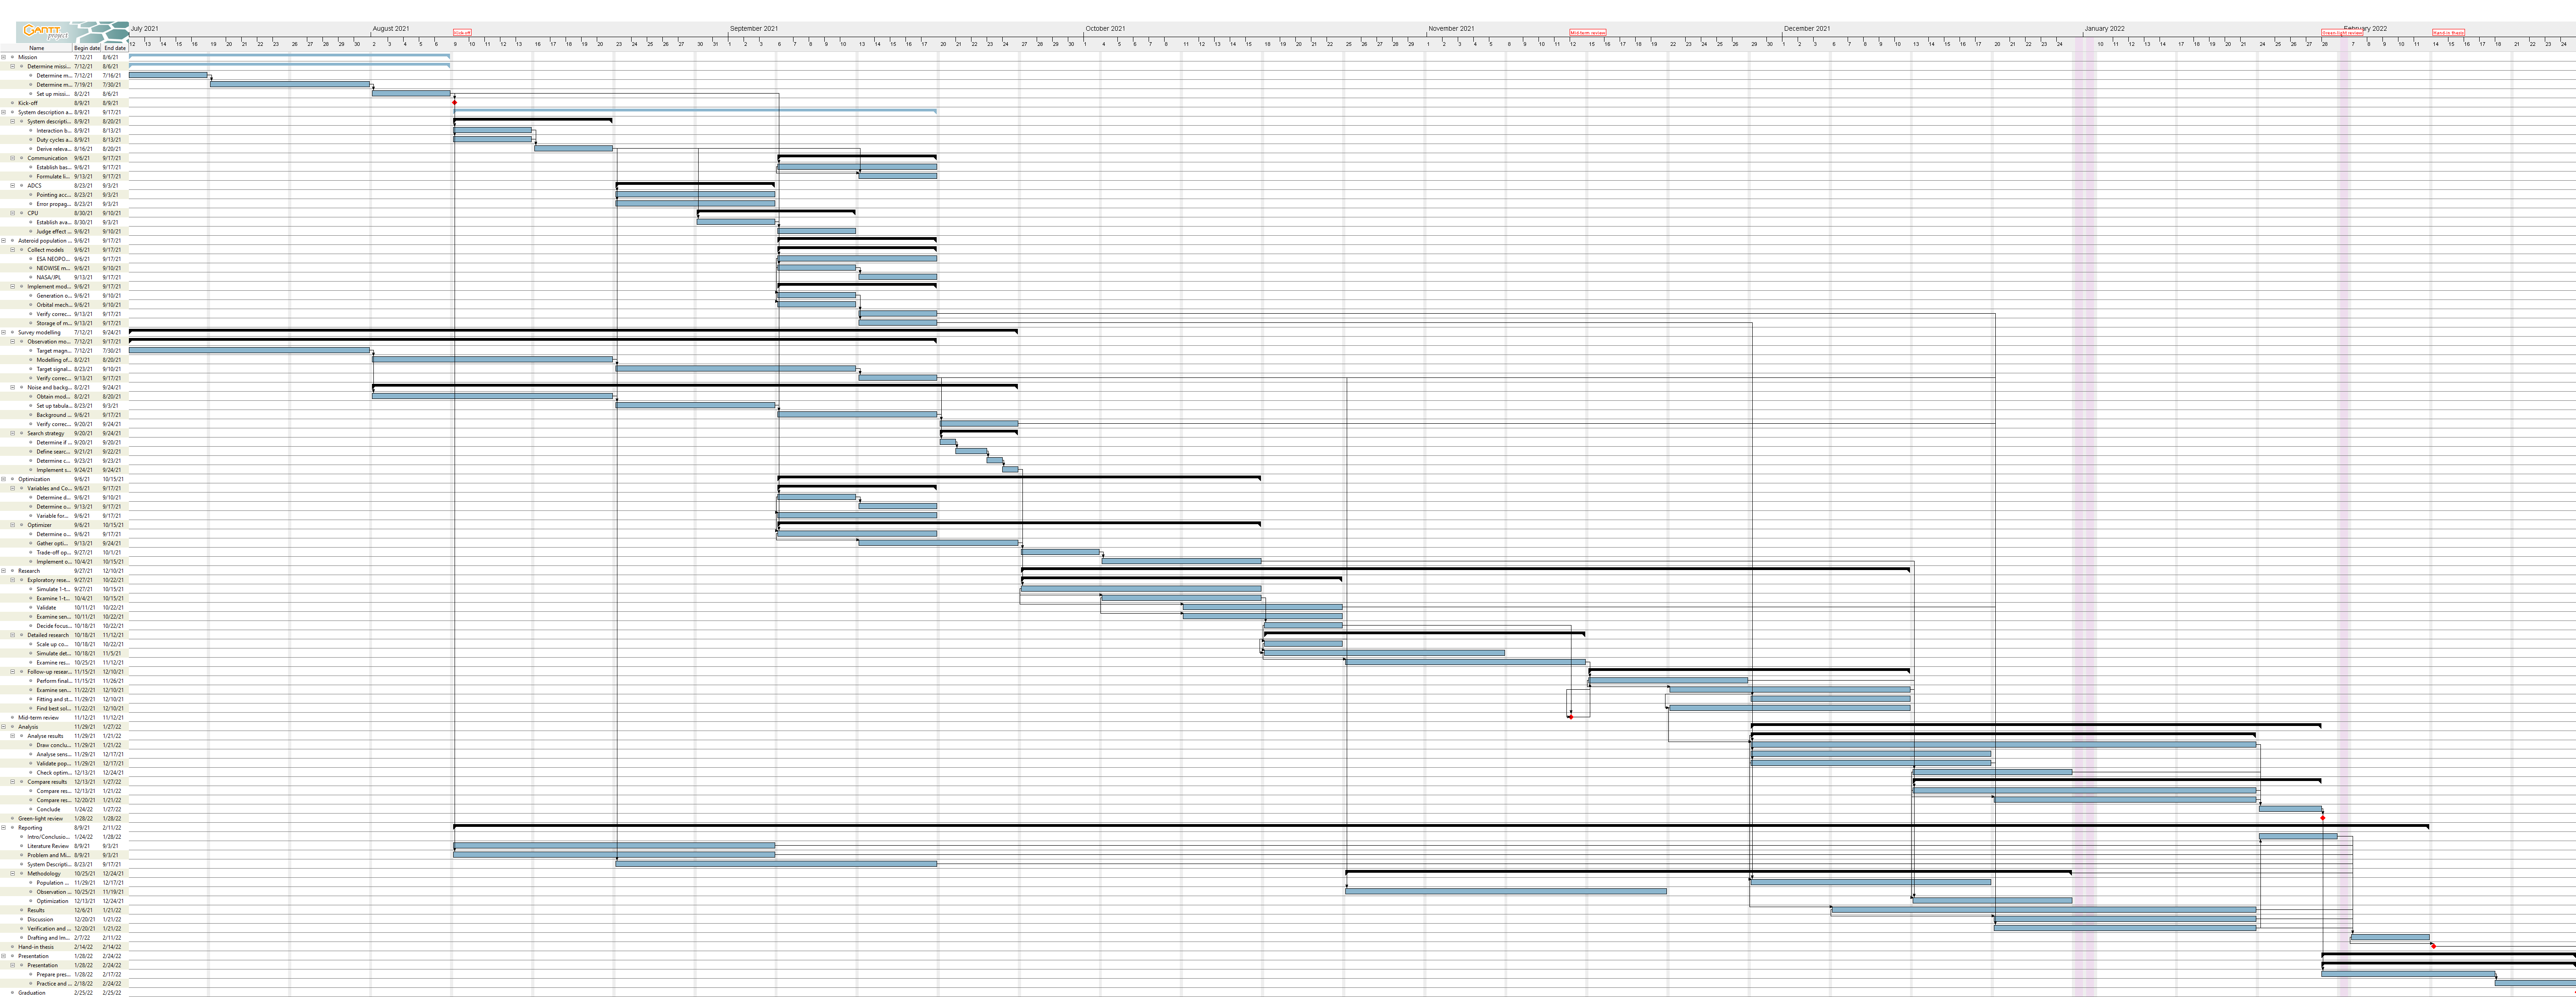
\includegraphics[width=1.0\textwidth]{figures/thesis_rm.png}
\end{figure}
Full resolution link: \url{https://surfdrive.surf.nl/files/index.php/s/PnEzMoALQzlE50b}
\end{landscape}
\end{document}
